% !TEX root = ../entropy.tex

\section{Spending profiles predict emergency savings}%
\label{sec:results}

Table~\ref{tab:reg_has_inflows_main} shows the effect of entropy on the
probability of building emergency savings in a given month. Columns (1)-(3)
show results for unsmoothed entropy based on 9 categories, 48 categories, and
merchant names, respectively. Columns (4)-(6) results for smoothed entropy
based on the same variables. All models include user and year-month fixed
effects, and standard errors are clustered at the user-level. 95\% confidence
intervals are shown in brakets.

\input{\tabdir/reg_has_inflows_main.tex}

Results for unsmoothed entropy suggest that a one unit increase in entropy is
associated with an increase in the probability of a user making at least one
transfer into their savings accounts of between 1.5 and 2.7 percentage points
-- an effect up to two times larger than that of a \pounds1000 increase in
monthly income. Conversely, the effect for unsmooth entropy is smaller in
magnitude but runs in the reverse direction: a one-unit increase in the
smoothed entropy score is associated with a reduction in the probability of
transferring money into savings account of between 0.4 and 1.6 percentage
points -- an effect that, in absolute magnitude, is about equal to that of a
\pounds1000 increase in monthly income.

As discussed in Section~\ref{sub:estimation}, these results are not a results
of reverse causality. While we might think that making a savings transactions
might change some or all of the components of entropy discussed in
Section~\ref{sub:spending_profiles} -- the number of unique spending categories
with positive frequency count, the standard deviation of these counts, and the
total number of spend transactions -- and thus change entropy, this is not the
case because of the way we define entropy and savings, and the way spending
transactions are categorised. We define entropy based on all current account
debits that are identified as spends, while we define savings transactions as
the sum of all savings accounts credits. If a user transfers money from their
current account to their savings account, this will be identified as a savings
transaction, but be identified as a transfer on their current account and thus
not considered when calculating their entropy score.

Overall, the effect of entropy in spending profiles is statistically and
economically significant, and robust across different definitions. In other
words, the scores seem to pick up a feature of the spending distribution that
is predictive of savings behaviour.

\edit{Two questions remain: first, how can we interpret the aspect of spending
distributions that entropy captures and that is related to savings behaviour?
Second, why does smoothing entropy scores flip the direction of the effec? We
will address these in turn.}


\subsection{Why does smoothing flip the direction of the effect}%
\label{sub:why_does_smoothing_flip_the_direction_of_the_effect}

One way to think about the sign change in Table~\ref{tab:reg_has_inflows_main}
is to realise that it implies that at least some individuals who used to have
high unsmoothed entropy must have low smoothed entropy and vice versa, so that
there is a large difference in the relative rank of their two entropy scores.
Hence, understanding who those individuals are might provide insights into both
the sign flip and into what entropy captures about spending behaviour.

To do this, it is useful to think of entropy as a function of a number of
simple components, and to rewrite Equation~\ref{equ:entropy} in a way that
makes this transparent. Let $\setcp = \{c: f_c > 0\}$ be the set of all
spending categories with positive frequency counts (i.e.  with at least one
transaction) and $\setcz = \{c: f_c = 0\}$ the set of all spending categories
with a zero frequency count, so that $\setc = \setcp \cup \setcz$. Then, using
our definitions of unsmoothed and smoothed probabilities above, we can write
unsmoothed entropy as

\begin{equation}
\label{equ:entropy_us}
H = -\sum_{c \in \setcp}{\left(\frac{f_c}{F}\right)
log\left(\frac{f_c}{F}\right)},
\end{equation}

and smoothed entropy as:

\begin{equation}
\label{equ:entropy_s}
H^s = -\sum_{c \in \setcp}{\left(\frac{f_c + 1}{F + |\setc|}\right)
log\left(\frac{f_c + 1}{F + |\setc|}\right)}
- |\setcz|\left(\frac{1}{F + |\setc|}\right)
log\left(\frac{1}{F + |\setc|}\right),
\end{equation}

\noindent where the size of set $\setcz$, $|\setcz|$, is the number of all
spending categories in which a user makes no transactions in a certain period.
These expressions make clear that, by definition, unsmoothed entropy is a
function of frequency counts of categories with positive counts only to avoid
taking logs of 0, while smoothed entropy has two parts: the additively smoothed
unsmoothed entropy, plus a constant term for each spending category with a zero
frequency count.

\edit{Maybe just talk about two components: non-zero counts and variation in
probabilities.}
The expressions also make transparent the three main components of both types
of entropy that are determined by user behaviour. The first is the number of
spending categories with a non-zero frequency count, $|\setcp|$, which
determines the number of elements summed over in Equation~\ref{equ:entropy_us},
and partitions the categories into either contributing to the sum on the left
hand side of Equation~\ref{equ:entropy_s} or to the constant term on the right
hand side since, for an exogenously fixed $|\setc|$, $|\setcz| = |\setc
\backslash \setcp|$ -- for a given number of total categories, the number of
categories with a zero frequency count is the difference between the total
number of categories and the number of categories with a positive frequency
count. The second component is the variation of the frequency counts, $f_c$,
which will determine the variation in the probabilities of a spend accurring in
a given category. The third component is the total number of transactions
($F$). The number of total spending categories, $|\setc|$, also determines
smoothed entropy and, implicitly, also unsmoothed entropy since it ``scales''
the number of categories with a positive frequency count, $|\setcp|$, as a
given number of spending transactions are categorised into finer or coarser
categories. But it is exogenously given and does not depend on user behaviour.

% As discussed in Section~\ref{sub:spending_profiles}, we create smooth entropy
% measures by additively smoothing the probabilities that a user makes a
% transaction in a particular spending category at a particular point in time. To
% do this, we add one to the frequency count of that spending category in the
% numerator and add the total number of spend categories to the total number of
% spend transactions in the denominator.

Equations~\ref{equ:entropy_us} and~\ref{equ:entropy_s} suggest two main sources
that might make smoothed entropy different from unsmoothed entropy in terms of
their relative ranks. First, we can see that the first part of smoothed entropy
that sums over all spending categories with positive frequency counts is very
similar to the entire expression of unsmoothed entropy -- it is that same
expression but with additively smoothed probabilities. Hence, all else equal,
the higher the number of categories with positive counts, the more smoothed
entropy is determined by that first part, and the more similar it will be to
unsmoothed entropy. As a result, we would expect to find large (rank)
differences between entropy scores among cases with a large number of
zero-count categories. Second, remember from
Section~\ref{sub:spending_profiles} that entropy is higher the more equal the
spending category probabilities are. Hence, for a given number of zero-count
categories, smoothed entropy will be higher if the (additively smoothed)
probabilities of all positive-count categories are close to the (additively
smoothed) probabilities of the zero-count categories, which will be the case
(i) if there are few overall transactions, such that counts frequency counts
($f_c$) are close to zero and (ii) if there is little variation in the counts.
Together, then, this suggests that we would expect entropy ranks to differ in
cases where an individual makes few spending purcheases overall and makes a similar
number of purchases in a small number of categories.

Figure~\ref{fig:scatter_facets} visualises this intuition for our 9-category
based entropy variable: it shows scatterplots of unsmoothed and smoothed
entropy separated by the number of categories with positive frequency counts
and coloured based on the standard deviation quintile of the frequency count
standard deviation. First, ignoring the colouring and focusing on the shape of
the dots only we can see that, as expected, the relationship between the two
entropy measures is tighter the higher the number of non-zero spending
categories is. The cases with large differences in relative entropy ranks are
to be found particularly in the top row. Among these, the colouring makes clear
that -- again as expected -- it is cases with similar frequency counts that
experience the largest change in entropy
rank.\footnote{Appendix~\ref{sub:entropy_correlations} shows similar plots
    coloured based on the standard deviation of counts and the total number of
    spend transactons.}

\begin{figure}[H]
    \centering 
    \caption{Effect of smoothing on entropy}
    \label{fig:scatter_facets}
    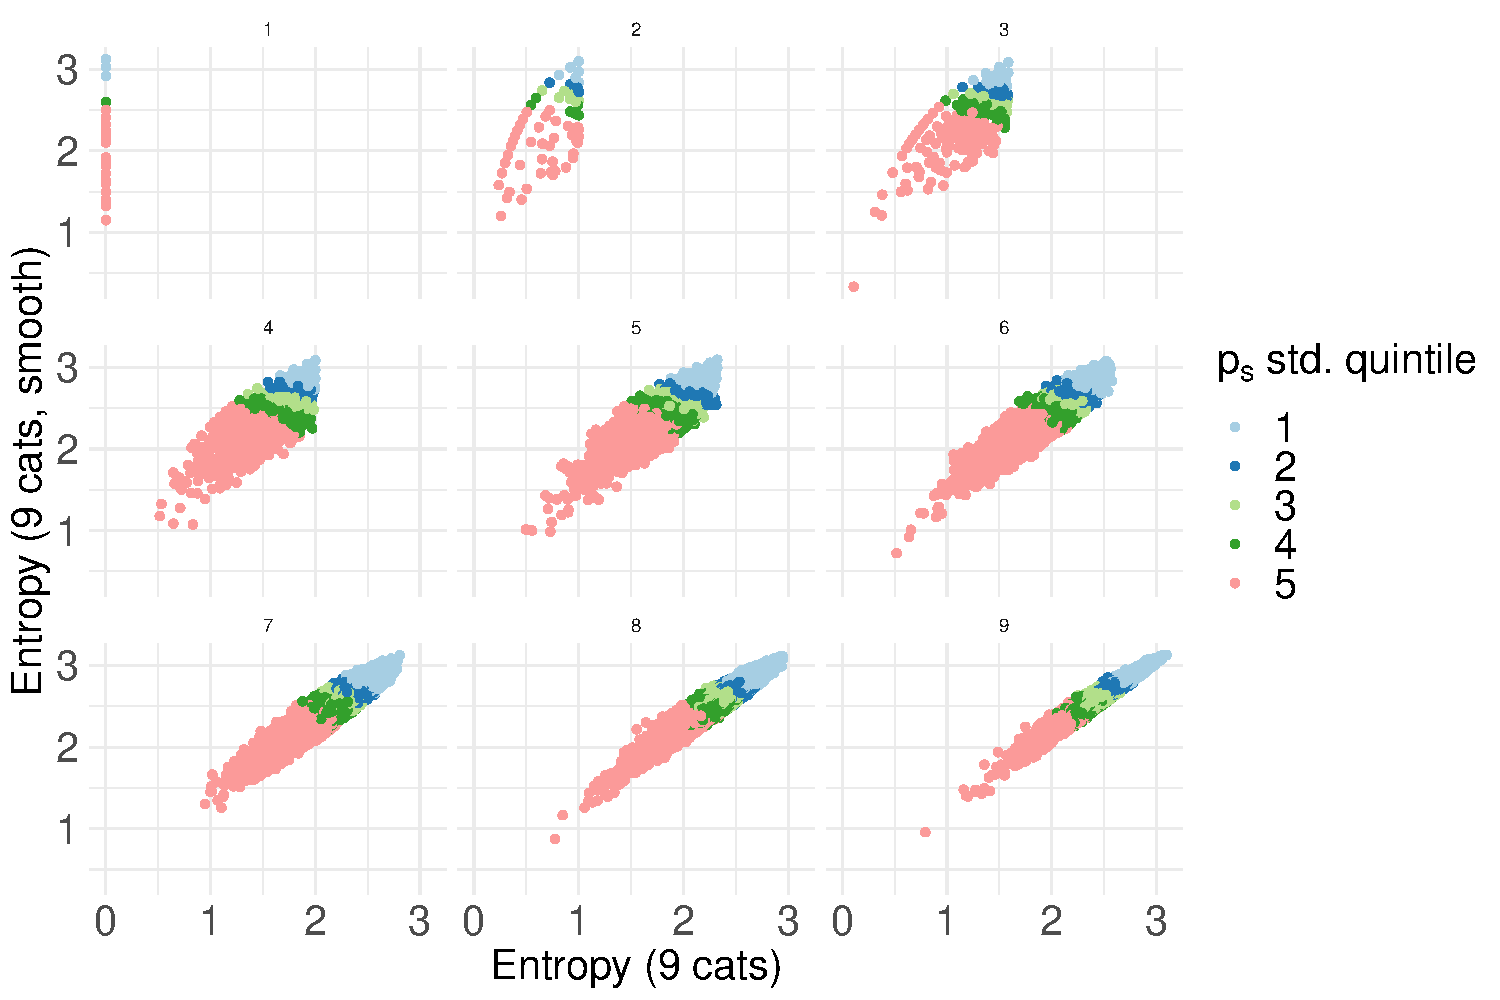
\includegraphics[width=\textwidth]{\figdir/scatter_facet_ps_std_q.png}
    % \fignote{\textwidth}{Effect of smoothing on entropy (top left) and entropy
    %     as a function of its three main components: the number of spending
    %     categories with positive frequency-counts (top right), the standard
    %     deviatioin of these counts (lower left), and the total number of
    % spending transaction (lower right). Value ranges for entropy components are
% trimmed at the 95th percentile.}
\end{figure}


\edit{Next: show number of spend profiles for users with high and low entropy
rank differences to undertand how they differ. Can we predict them based on
other features in teh data?}


\begin{table}[htbp]
   \centering
   \tiny
   \begin{threeparttable}[b]
      \caption{\label{tab:reg_comp_only} Disaggregating entropy into components}
      \begin{tabular}{lcccc}
         \tabularnewline \midrule \midrule
          & \multicolumn{2}{c}{Entropy (48 cats)} & \multicolumn{2}{c}{Entropy (48 cats, smooth)} \\ 
         Model:               & (1)              & (2)              & (3)              & (4)\\  
         \midrule
         \emph{Variables}\\
         Unique categories    & 0.090$^{***}$    & 0.088$^{***}$    & -0.014$^{***}$   & -0.015$^{***}$\\   
                              & [0.090; 0.090]   & [0.087; 0.088]   & [-0.014; -0.013] & [-0.017; -0.012]\\   
         Category counts std. & -0.292$^{***}$   & -0.287$^{***}$   & -0.509$^{***}$   & -0.473$^{***}$\\   
                              & [-0.293; -0.292] & [-0.294; -0.281] & [-0.510; -0.508] & [-0.484; -0.462]\\   
         Number of spend txns & 0.013$^{***}$    & 0.013$^{***}$    & 0.012$^{***}$    & 0.010$^{***}$\\   
                              & [0.013; 0.013]   & [0.013; 0.013]   & [0.012; 0.012]   & [0.009; 0.011]\\   
         (Intercept)          & -0.706$^{***}$   &                  & 0.982$^{***}$    &   \\   
                              & [-0.707; -0.704] &                  & [0.979; 0.984]   &   \\   
         \midrule
         \emph{Fixed-effects}\\
         User                 &                  & Yes              &                  & Yes\\  
         Year-month           &                  & Yes              &                  & Yes\\  
         \midrule
         \emph{Fit statistics}\\
         Observations         & 1,043,727        & 1,043,727        & 1,043,727        & 1,043,727\\  
         R$^2$                & 0.84686          & 0.90609          & 0.86248          & 0.92337\\  
         Within R$^2$         &                  & 0.77476          &                  & 0.81733\\  
         \midrule \midrule
         \multicolumn{5}{l}{\emph{Signif. Codes: ***: 0.01, **: 0.05, *: 0.1}}\\
      \end{tabular}
   \end{threeparttable}
\end{table}



% Negative sign in 4 makes sense: since increading f_c moves fraction closer to
% one, moves log closer to zero, hence, H^s increases more if c added to rhs of
% expression.

% \begin{figure}[H]
%     \centering 
%     \caption{Effect of smoothing on entropy}
%     \label{fig:effect_of_smoothing}
%     \includegraphics[width=.49\textwidth]{\figdir/smoothed_unsmoothed_corr.png}
%     \includegraphics[width=.49\textwidth]{\figdir/smoothing_on_nunique_tag_spend.png}
%     \includegraphics[width=.49\textwidth]{\figdir/smoothing_on_std_tag_spend.png}
%     \includegraphics[width=.49\textwidth]{\figdir/smoothing_on_txns_count_spend.png}
%     % \fignote{\textwidth}{Effect of smoothing on entropy (top left) and entropy
%     %     as a function of its three main components: the number of spending
%     %     categories with positive frequency-counts (top right), the standard
%     %     deviatioin of these counts (lower left), and the total number of
%     % spending transaction (lower right). Value ranges for entropy components are
% % trimmed at the 95th percentile.}
% \end{figure}

The two salient facts from the top left panel are that unsmoothed and smoothed
entropy are positively correlated, and that the variance of smoothed entropy
scores for any given level of unsmoothed entropy decreases as unsmoothed
entropy gets larger.

This makes sense: correlates positively becuase first part of smoothed entropy
is almost equal to unsmoothed entropy. Higher variance for lower levels of
unsmoothed entropy because it is low if there are many spend categories with zero
counts, which do not enter the sum. However, in smoothed entropy, all these
categories contribute to the constant part on the right hand side. Depending on
other elements of the distribution, this creates a high or low smoothed entropy
score.


\subsection{How can we interpret entropy?}%
\label{sub:is_entropy_more_than_the_sum_of_its_parts_}

One possibility is that spending entropy is related to savings behaviour
through some or all of its main components we discussed in
Section~\ref{sub:spending_profiles}: the number of unqiue spending categories
with a positive frequency count, the standard deviation of those counts, and
the number of spending transactions. Here we want to test whether entropy
remains predictive of savings behaviour once we control for these components.


\begin{table}[htbp]
   \centering
   \tiny
   \begin{threeparttable}[b]
      \caption{\label{tab:reg_has_inflows_comp} Controlling for entropy components}
      \begin{tabular}{lcccc}
         \tabularnewline \midrule \midrule
         Model:                    & (1)             & (2)             & (3)              & (4)\\  
         \midrule
         \emph{Variables}\\
         Entropy (48 cats)         & 0.029$^{***}$   & 0.013$^{***}$   &                  &   \\   
                                   & [0.025; 0.033]  & [0.006; 0.021]  &                  &   \\   
         Entropy (48 cats, smooth) &                 &                 & -0.023$^{***}$   & -0.028$^{***}$\\   
                                   &                 &                 & [-0.025; -0.020] & [-0.034; -0.022]\\   
         Unique categories         &                 & 0.004$^{***}$   &                  & 0.004$^{***}$\\   
                                   &                 & [0.003; 0.005]  &                  & [0.004; 0.005]\\   
         Category counts std.      &                 & 0.002           &                  & -0.015$^{***}$\\   
                                   &                 & [-0.001; 0.006] &                  & [-0.018; -0.011]\\   
         Number of spend txns      &                 & 0.000$^{***}$   &                  & 0.001$^{***}$\\   
                                   &                 & [0.000; 0.001]  &                  & [0.001; 0.001]\\   
         Month spend               & 0.009$^{***}$   & 0.005$^{***}$   & 0.008$^{***}$    & 0.005$^{***}$\\   
                                   & [0.008; 0.009]  & [0.004; 0.006]  & [0.007; 0.009]   & [0.005; 0.006]\\   
         Month income              & 0.012$^{***}$   & 0.011$^{***}$   & 0.011$^{***}$    & 0.011$^{***}$\\   
                                   & [0.011; 0.013]  & [0.010; 0.012]  & [0.011; 0.012]   & [0.010; 0.012]\\   
         Has income in month       & 0.084$^{***}$   & 0.079$^{***}$   & 0.085$^{***}$    & 0.078$^{***}$\\   
                                   & [0.075; 0.092]  & [0.070; 0.087]  & [0.076; 0.093]   & [0.070; 0.087]\\   
         Income variability        & 0.001$^{*}$     & 0.000           & 0.001$^{*}$      & 0.000\\   
                                   & [-0.000; 0.001] & [-0.000; 0.001] & [-0.000; 0.001]  & [-0.000; 0.001]\\   
         \midrule
         \emph{Fixed-effects}\\
         User                      & Yes             & Yes             & Yes              & Yes\\  
         Year-month                & Yes             & Yes             & Yes              & Yes\\  
         \midrule
         \emph{Fit statistics}\\
         Observations              & 1,043,727       & 1,043,727       & 1,043,727        & 1,043,727\\  
         R$^2$                     & 0.45395         & 0.45498         & 0.45415          & 0.45515\\  
         Within R$^2$              & 0.00768         & 0.00956         & 0.00805          & 0.00986\\  
         \midrule \midrule
         \multicolumn{5}{l}{\emph{Clustered (User) co-variance matrix, 95\% confidence intervals in brackets}}\\
         \multicolumn{5}{l}{\emph{Signif. Codes: ***: 0.01, **: 0.05, *: 0.1}}\\
      \end{tabular}
   \end{threeparttable}
\end{table}




Columns (1) and (3) in Table~\ref{tab:reg_has_inflows_comp} replicate the
results for the 48-category-based unsmoothed and smoothed entropy measures
presented in Table~\ref{tab:reg_has_inflows_main} for reference. In columns (2)
and (4) we additionally control for the three entropy components. Including
these components has some effect: for unsmoothed entropy the magnitude of the
coefficient is less than half its size and the confidence interval is about
twice as wide, while for smoothed entropy the magnitude of the coefficient is a
little higher while the width of the confidence interval also roughly doubles.
However, both coefficients remain statistically significant and their
confidence intervals cover values that are also economically significant.
Hence, the results make clear that the results in
Table~\ref{tab:reg_has_inflows_main} cannot be attributed simply to the effect
of one or more of entropy's simple components.

Knowing that entropy is not simply the sum of its component parts still leaves
us with the question what it \textit{is} that entropy captures about user
spending distributions that is predictive of savings behaviour. We have not,
thus far, been able to understand this and leave the question for future
research.



